\section{FAT}
\subsection{Introducción}
\begin{frame}{Introducción}
  \begin{itemize}
    \item Creado por Bill Gates y Marc McDonald.
    \item Se creo en 1977.
    \item Su primera version fue FAT12 (con direciones de 12 bits).
    \item Posteriormente aparecio FAT16.
    \item Finalmente se llego a FAT32 (el actual) (28 bits).
  \end{itemize}
\end{frame}

\subsection{Caracteristicas}
\begin{frame}{Caracteristicas}
  \begin{itemize}
    \item Tamaño maximo: 32GB
    \item Tamaño maximo de fichero: 4GB
    \item Maximo de caracteres de nombre de fichero: 255B
    \item Maximo numero de ficheros: 4.177.920
  \end{itemize}
\end{frame}

\subsection{Estructura}
\begin{frame}{Estructura}
  \begin{itemize}
    \item Al principio de la particion nos encontramos el sector de arranque.
    \item Justo despues se encuentra la FAT
    \item Normalmente (pero no necesariamente) encontramos despues el directorio raiz.
    \item Despues nos encontramos el area de datos, donde se almacenan todos los ficheros.
  \end{itemize}
\end{frame}

\begin{frame}{Estructura}
  \begin{center}
    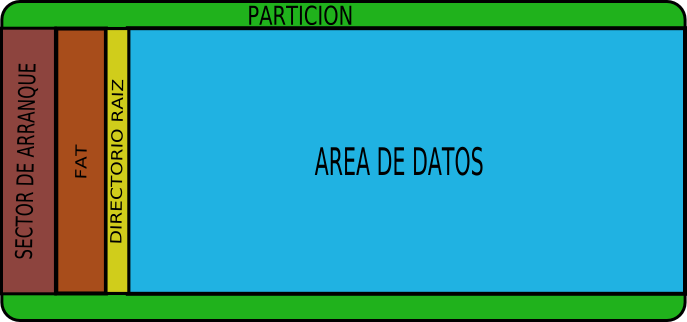
\includegraphics[height=5.5cm]{imgs/fat_struct.png}
  \end{center}
\end{frame}

\begin{frame}{Ficheros}
  \begin{itemize}
    \item Los ficheros unica y exclusivamente contienen datos y estan almacenados en el sector de datos de la particion.
    \item Las entradas de directorios almacenan el nombre, el numero de cluster y los atributos de cada uno de los ficheros que contiene.
    \item Los ficheros vacios no contienen ocupan bloques de datos ni entradas en la fat.
    \item Si un cluster no es el ultimo del fichero, contiene el numero de cluster siguiente, si lo es, contiene una marca.
    \item Los directorios siempre contiene como minimo los subdirectorios "." y "..", excepto el directorio raiz.
  \end{itemize}
\end{frame}

\begin{frame}{Ficheros}
  \begin{center}
    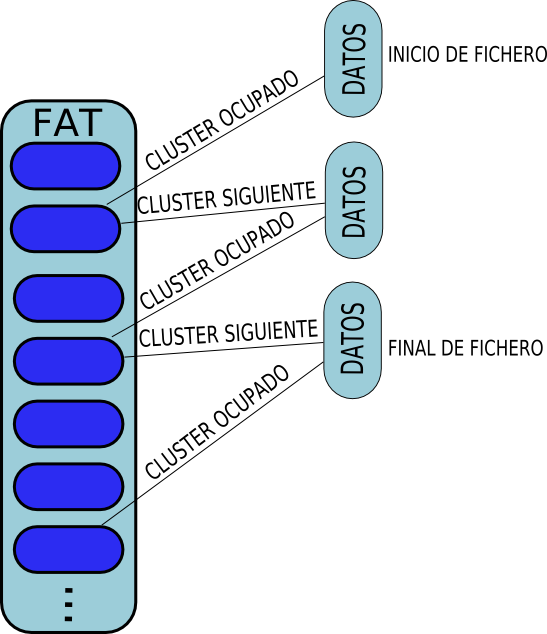
\includegraphics[height=6cm]{imgs/fat_files.png}
  \end{center}
\end{frame}
